\subsection{Casos de prueba}

Para verificar el correcto funcionamiento del algoritmo utlizamos los siguientes casos de prueba:

\begin{figure}[H]
 \centering
  \subfloat[9 servidores conectados.]{
   \label{}
    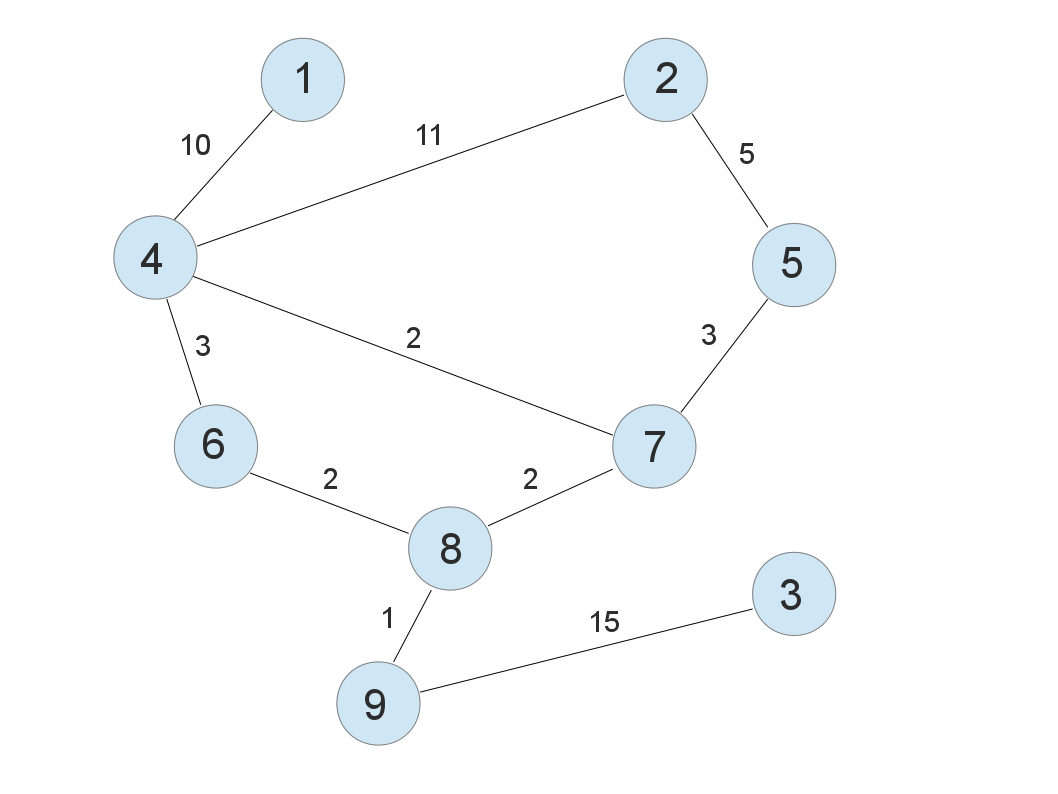
\includegraphics[scale=0.3]{ej3/imgs/graph_test1.png}}
  \subfloat[9 servidores conectados.]{
   \label{}
    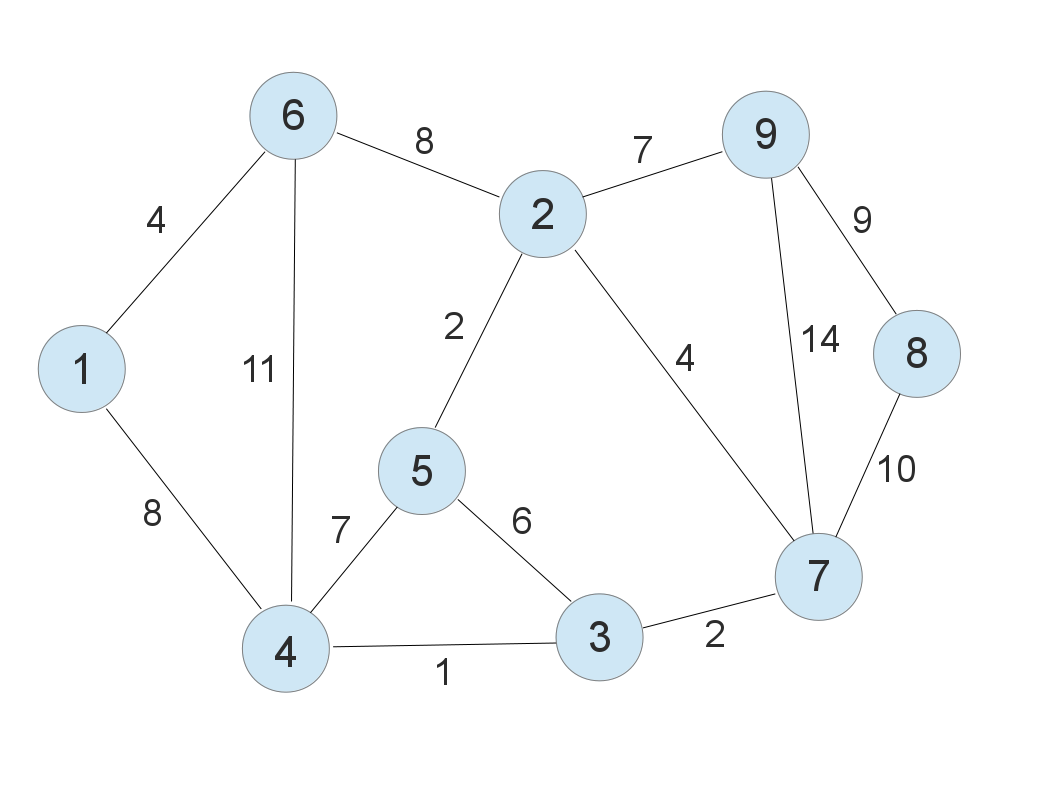
\includegraphics[scale=0.3]{ej3/imgs/graph_test4.png}}
 \caption{Casos de prueba}
 \label{}
\end{figure}

Las soluciones fueron:

\begin{figure}[H]
 \centering
  \subfloat[Costo toal: 40]{
   \label{}
    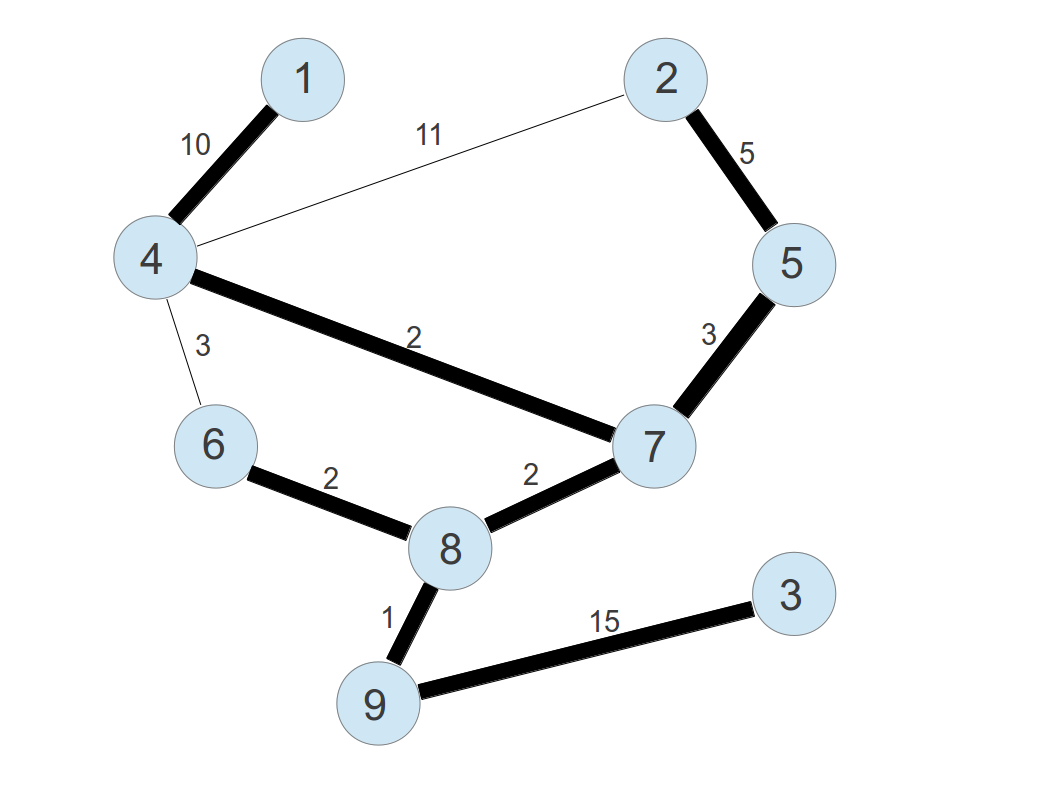
\includegraphics[scale=0.3]{ej2/1/imgs/graph_test1_sol.png}}
  \subfloat[Costo total: 37]{
   \label{}
    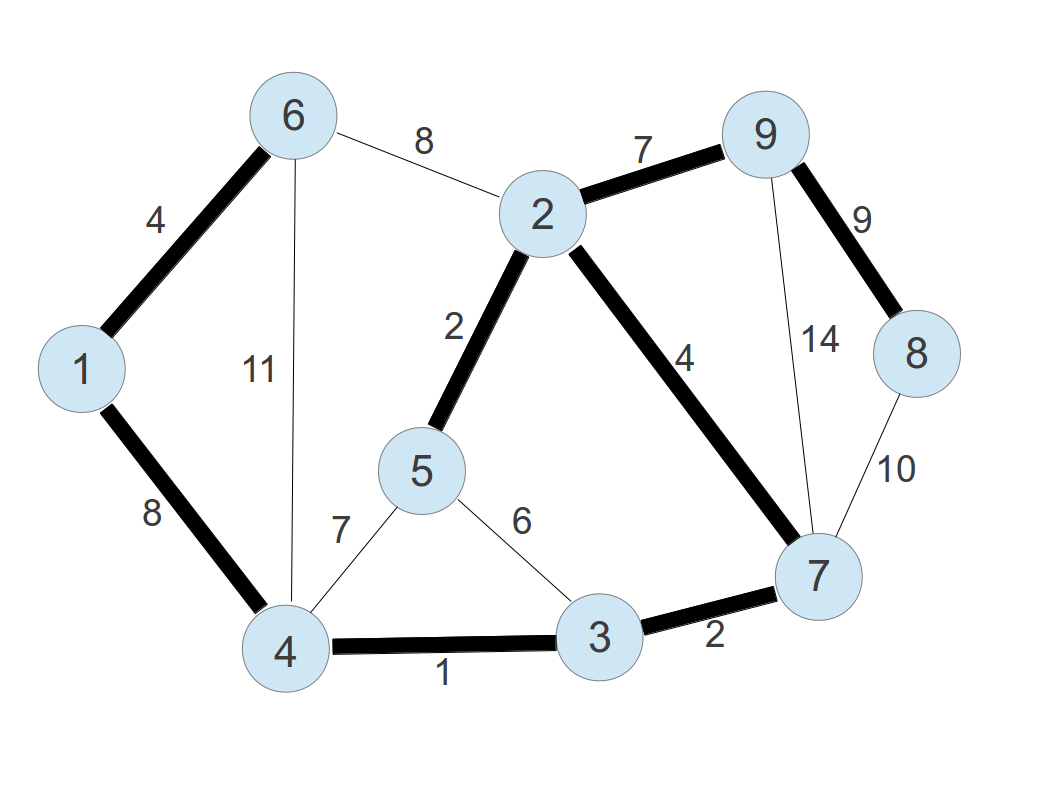
\includegraphics[scale=0.3]{ej2/1/imgs/graph_test4_sol.png}}
 \caption{Casos de prueba}
 \label{}
\end{figure}

Las soluciones halladas efectivamente son AGM's.

